% Post-hoc follow-ups (9 Nov 2026), run after the main results and the progress check.
% Numbers: results/final/followup_*; scripts/followup_headroom.py and scripts/followup_check_quality.py.
\clearpage  % place the ablation table before this section
\section{Post-hoc Follow-ups}
\label{app:followups}

Both follow-ups were added after the main results, so they are post-hoc and do not replace the
frozen extension. Each was gated only on the validation split, with a go/no-go criterion fixed in
its code before running: it goes to the test split only if it beats the relevant baselines by at
least three of the 40 validation questions, averaged over seeds 1--3. Both use at most 14 calls per question, the same budget as search and best-of-$N$.

\paragraph{Seeding fix (21 Nov).} In our final review we found that repeated sampled requests used server seed $s + i$ for run seed $s$ and sample $i$, so seeds 1--3 of best-of-$N$ and of this appendix's methods shared most of their samples. We now step sampled requests by 1000 ($s + 1000i$), added a test that seeds 1--3 never share a server seed, and re-ran every affected run (best-of-$N$ and structured + vote, capped and uncapped, in Tables~\ref{tab:main-results} and~\ref{tab:followups}, and the validation runs below). Calls issued once per question, which include all greedy calls and the search's proposals, keep their server seed, so search, direct generation and structured prompting replay identically. The superseded runs are kept in \texttt{results/superseded\_overlapping\_seeds/}; no conclusion changed.

\paragraph{Voting with an applicability check (did not pass).}
Most wrong best-of-$N$ answers are inapplicable actions (66 to 71 of 130 per seed). At least one of
the 14 samples is correct in about half of the test questions, and voting over only the truly
applicable samples would reach about 0.37. The search's predictor rarely says NOT APPLICABLE: it catches
14\% of the inapplicable root candidates (108 of 781). We therefore sampled 11 answers and asked the
LLM to check the preconditions of the three most-voted actions in turn, answering with the first
one it accepted. On the validation split it was correct on 8, 9 and 11 of 40 questions against 12, 12 and 10 for best-of-$N$ ($N{=}14$), so it did not go to the test split. The check caught 78\% of the inapplicable actions but also rejected 40\% of the applicable ones, discarding correct answers.
Like its progress scores, the LLM's applicability judgments are too unreliable to filter its own
candidates.

\paragraph{Structured prompting with majority vote (passed).}
This combines the two strongest baselines on test (on validation, direct scored 10/40, greedy structured prompting 9/40 and best-of-$N$ 12, 12 and 10, so the idea came from the test results and only its go/no-go from validation): it samples the structured prompt 14 times at temperature
0.7 and returns the most common final action, which is self-consistency~\citep{wang2023selfconsistency} applied to the structured prompt. On the validation split it was correct on 16, 16 and 18 of 40 questions, against 11.3 on average for best-of-$N$ and 9 for greedy structured prompting.
Table~\ref{tab:followups} gives the test results. With 14 calls it reaches $0.331 \pm 0.027$, the best result in this project (against the paper's single-call 0.25, one-sample binomial $p = 0.09$, $0.004$, $0.09$). It is higher than direct generation in every seed ($p = 0.043, 0.005, 0.058$, exact McNemar) and than best-of-$N$ ($p = 0.043, 0.002, 0.136$), and higher than greedy structured prompting, but significantly so only in seed 2 ($p = 0.143, 0.019, 0.248$). It uses 27\% more tokens than best-of-$N$ (29,080 against 22,960 per question). Under the 14,000-token cap it still leads ($0.321 \pm 0.012$ against 0.210, $p = 0.004, 0.043, 0.029$); the capped runs replay the first samples of the uncapped ones, so they are a truncation, not a replication. The cap is checked before each call and its calls are long, so it exceeds the cap on 129 to 130 of the 130 questions (15,036 tokens on average, against 12,348 for best-of-$N$, which exceeds it on 35). With a budget fixed per question in advance, giving each question only as many samples as fit in the tokens capped best-of-$N$ used on it (5.6 samples, 11,495 tokens on average), it still reaches $0.313$ (seeds 0.315, 0.323, 0.300). The gain
comes from sampling and voting over explicit reasoning, not from search, which is consistent with
our main finding that the LLM's judgments of its own candidates are the bottleneck.

\begin{table}[!ht]
\centering
\caption{Post-hoc follow-up on the test split (130 questions, seeds 1--3 for sampled methods). The 70B
structured, best-of-$N$ and structured + vote runs were pre-registered on 22 Nov; 70B direct and search are the main runs. Generated by \texttt{experiments/followups.py}.}
\label{tab:followups}
\small
\begin{tabular}{@{}lccc@{}}
\toprule
Method & Accuracy & Calls & Tokens \\
\midrule
\multicolumn{4}{@{}l}{\emph{Llama 3.1 8B}} \\
Direct generation & 0.223 & 1.0 & 1,640 \\
Structured prompting & 0.262 & 1.0 & 2,076 \\
Best-of-N ($N{=}14$) & 0.231 $\pm$ 0.015 & 14.0 & 22,960 \\
Search & 0.159 $\pm$ 0.012 & 13.4 & 13,722 \\
\textbf{Structured + vote} ($N{=}14$) & \textbf{0.331 $\pm$ 0.027} & 14.0 & 29,080 \\
\midrule
Best-of-N ($N{=}8$), 14k-token cap & 0.210 $\pm$ 0.016 & 7.7 & 12,348 \\
Search, 14k-token cap & 0.151 $\pm$ 0.018 & 12.2 & 11,230 \\
Structured + vote, 14k-token cap & 0.321 $\pm$ 0.012 & 7.5 & 15,036 \\
\midrule
\multicolumn{4}{@{}l}{\emph{Llama 3.1 70B}} \\
Direct generation & 0.377 & 1.0 & 1,645 \\
Structured prompting & 0.469 & 1.0 & 1,991 \\
Best-of-N ($N{=}14$) & 0.364 $\pm$ 0.016 & 14.0 & 23,032 \\
Search & 0.362 $\pm$ 0.015 & 11.4 & 10,292 \\
\textbf{Structured + vote} ($N{=}14$) & \textbf{0.492 $\pm$ 0.013} & 14.0 & 28,165 \\
\bottomrule
\end{tabular}
\end{table}


\paragraph{Repeat on 70B (pre-registered).} The 8B follow-up and controls were repeated unchanged on Llama~3.1~70B, with the methods, seeds and tests fixed in \texttt{experiments/preregistration\_22nov.md} before any run. Structured + vote reaches $0.492 \pm 0.013$ (66, 63 and 63 of 130), above best-of-$N$ at the same 14 calls ($0.364 \pm 0.016$; $p = 0.0003, 0.006, 0.02$) and above direct generation ($0.377$; $p = 0.002, 0.007, 0.016$). It is above the paper's 70B value of 0.42 in every seed, though not significantly even when that value is treated as exact ($p = 0.05$, $0.15$, $0.15$). Most of the gain comes from the structured prompt: one greedy structured call scores $0.469$ ($p = 0.05$ against direct), and voting adds $+0.023$ (not pre-registered; seeds pooled $p = 0.50$, per seed $p \ge 0.33$). As at 8B, best-of-$N$ is no better than direct generation ($p = 0.22$, $1.0$, $1.0$), and search ($0.362$) is no better than either. The first launch of these runs (22 Nov, 22:55, after the pre-registration commit at 22:52) was stopped by an API spending cap; the re-launch replayed its cached calls, so no answer changed and no run was discarded. These runs were scored with the re-checking validator of D8.

\begin{figure}[ht]
\centering
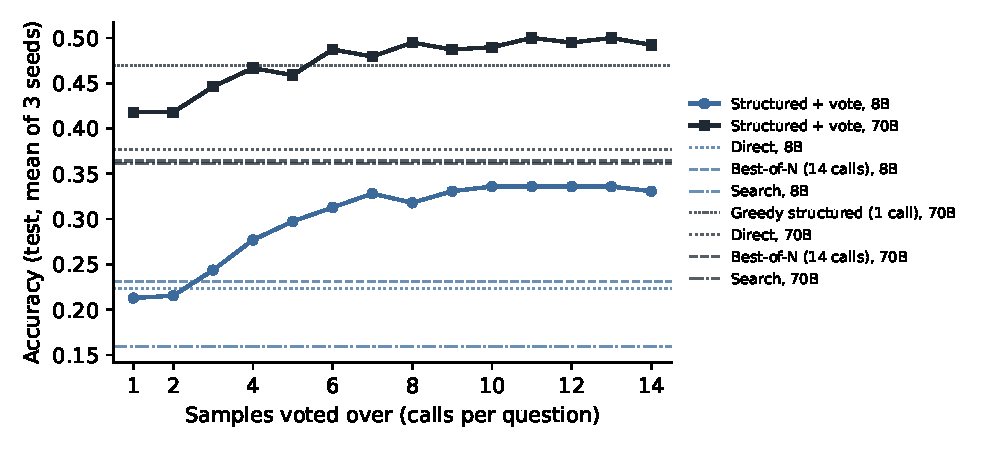
\includegraphics[width=0.95\linewidth]{figures/vote_curve.pdf}
\caption{Structured + vote accuracy against the number of samples voted over (test, mean of seeds 1--3; voting over each run's first $m$ samples), with the 14-call best-of-$N$, direct generation, search and, for 70B, one greedy structured call as reference lines. Generated by \texttt{experiments/followups.py}.}
\label{fig:vote-curve}
\end{figure}

\paragraph{Seed-pooled tests.} The McNemar tests above are per seed and uncorrected. Pooling the seeds, we average each question's correctness over seeds 1--3 and run a paired sign-flip permutation test with a bootstrap 95\% interval on the mean difference (\texttt{experiments/followups.py}). Best-of-$N$ beats search by $+0.072$ ($[+0.008, +0.138]$, $p = 0.04$); search against direct generation gives $-0.064$ ($p = 0.08$) for 8B and $-0.015$ ($[-0.09, +0.06]$, $p = 0.73$) for 70B. Under the token cap, best-of-$N$ against search gives $+0.059$ ($p = 0.08$). Structured + vote beats direct generation by $+0.108$ ($p = 0.008$), best-of-$N$ by $+0.100$ ($p = 0.003$) and greedy structured prompting by $+0.069$ ($p = 0.03$); capped, it beats capped best-of-$N$ by $+0.110$ ($p < 0.001$). Fixed scoring against the frozen search gives $+0.031$ ($p = 0.10$), and best-of-$N$ against direct generation $+0.008$ ($p = 0.83$). These tests are uncorrected, and the test is approximate when a three-seed mean is compared with a single greedy run. With a Holm correction over all twelve, including the two 70B tests (the pre-registered primary test, structured + vote against best-of-$N$, $p = 0.0008$, and against direct generation, $p = 0.002$), four stay below 0.05: structured + vote against best-of-$N$ at 8B, capped and uncapped, and both 70B tests. Resampling the 13 domains instead of questions (not pre-registered; with 13 clusters, approximate), to allow for questions of one domain being correlated, keeps every one of these intervals above zero (8B against best-of-$N$: $[+0.04, +0.17]$, capped: $[+0.04, +0.18]$; 70B: $[+0.05, +0.21]$).

\paragraph{Prompt and generated tokens.} The token counts include the prompt of every call. Per question, best-of-$N$ uses 22,797 prompt and 163 generated tokens, search 11,852 and 1,870, structured + vote 24,141 and 4,939, and direct generation 1,628 and 12. Best-of-$N$'s extra tokens are the same prompt sent 14 times, so in generated tokens search costs about 11 times as much as best-of-$N$; structured + vote generates about 30 times as much as best-of-$N$, and about 400 times as much as direct generation.
